\chapter{Uncertainty and Error Part 2}
\label{chap:excel2}
\section{Introduction}

The purpose of this lab is to introduce some more advanced topics in error analysis and excel as an extension to the first lab.You will perform two experiments, demonstrating how we can use the principles of error analysis and excel to analyze data in real experiments. The techniques studied here will be essential for the rest of this two-semester lab course. The issues and techniques are important in order to arrive at accurate conclusions in any field in which it is necessary to understand not just numerical results, but the uncertainties associated with those results. \myskip

If you wish to use your personal laptop and have not already acquired a copy of Excel, you can download a copy with your student email address from 
\href{https://products.office.com/en-us/student?ms.officeurl=getoffice365}{Office 365 Education}\footnote{https://products.office.com/en-us/student?ms.officeurl=getoffice365}. However, this will not be absolutely necessary since computers are provided in the laboratory. Please note the sections introducing new Excel tools pertain to the newest version of Excel. If you are using a personal computer with a different version of Excel, you are responsible for adapting the instructions to your version of Excel.


\section{Theory}
\subsection{Advanced Uncertainty and Error}
\subsubsection{Powers and Roots}

When raising a value to a certain power, its relative uncertainty is multiplied by the exponent. This applies to roots as well, since taking the root of a number is equivalent to raising that number to a fractional power.\myskip 

Squaring a quantity involves multiplying its relative uncertainty by 2, while cubing a quantity causes its relative uncertainty to be multiplied by 3.\myskip

Taking the \underline{square root} of a quantity (which is equivalent to raising the quantity to the 1/2 power) causes its \underline{relative uncertainty} to be multiplied by 1/2. For example, if you know the area of a square to be: 
\begin{equation}
    \text{Area} = 100\pm 8\,\mathrm{m^2} = 100\,\mathrm{m}^2\;(1.00\pm 0.08)
\end{equation}
then it follows that the side of the square is:
\begin{equation}
    \text{Side} = 10\,\mathrm{m}\;\left( 1.00\pm 0.04 \right) = 10.0\pm 0.4\,\mathrm{m}
\end{equation}
The most general rule for finding the error in powers and roots is mathematically represented as follows.
\begin{gather}
f(x) = x^n \\
\frac{\sigma_{f(x)}}{f(x)} = |n| \frac{\sigma_x}{x}
\end{gather}
Where $\sigma$ is the {\it{absolute}} uncertainty and $f(x)$ is some power or root of $x$.
You can convince yourself that this is true by checking it backwards using the rules described in section 2.6.2 in the previous chapter (chapter 1-\ref{chap:excel}).

\subsubsection{Other Functions}

If you need to calculate the error of a calculation that does not fit into one of these rules (such as trigonometric functions or logarithmic ones), here is a manual method that you can use.\myskip

Based upon the error of the quantity that you determined, you can find the maximum and minimum values of the quantity that you are calculating. The value that you found should be roughly midway between these two quantities. Then if you split the difference between the maximum and minimum you should obtain a reasonable estimate of the error. Mathematically, you would do so as follows.
\begin{gather}
\sigma_{f(x)} = \frac{f(x + \sigma_x) - f(x - \sigma_x)}{2}
\end{gather}

Here is an example: Suppose you measure an angle to be $(47.3 \pm 0.5)^\circ$ and you want to determine the error of $\sin(47.3 \pm 0.5)^\circ$. You find that $\sin(47.3) = 0.735$. Based upon your reported uncertainty, you know that your angle could be as large as $47.8^\circ$ and as small as $46.8^\circ$, and therefore you should calculate $\sin(47.8) = 0.741$ and $\sin(46.8) = 0.729$. So your calculated value is 0.735 but it can be as low as 0.729 and as high as 0.741 and therefore, if you halve the difference between 0.729 and 0.741 you get a reasonable error estimate of 0.006. So you should report your value as $0.735 \pm 0.006$.

\subsubsection{Best-Fit Line}

In most research laboratories, plotting measurements is found to be the preferred method of reviewing the data and quantitatively measuring the relationship between the experimental variables. This is effective because we often have some idea of the expected relationship between the variables {\it{apriori}}. In these labs, this expected relationship is almost always arranged to be a straight line. But even if we know that the ideal points fit on a precise straight line, experimentally measured data points will not always lie on a single line -- because the measurements always have intrinsic uncertainty. Therefore when the points are plotted, we should include error bars on both axes to indicate the uncertainties in the data. Because real measurements do not all lie on a single straight line, there are a variety of possible lines you might choose to fit the data. \myskip

\begin{figure}[h]
    \begin{center}
        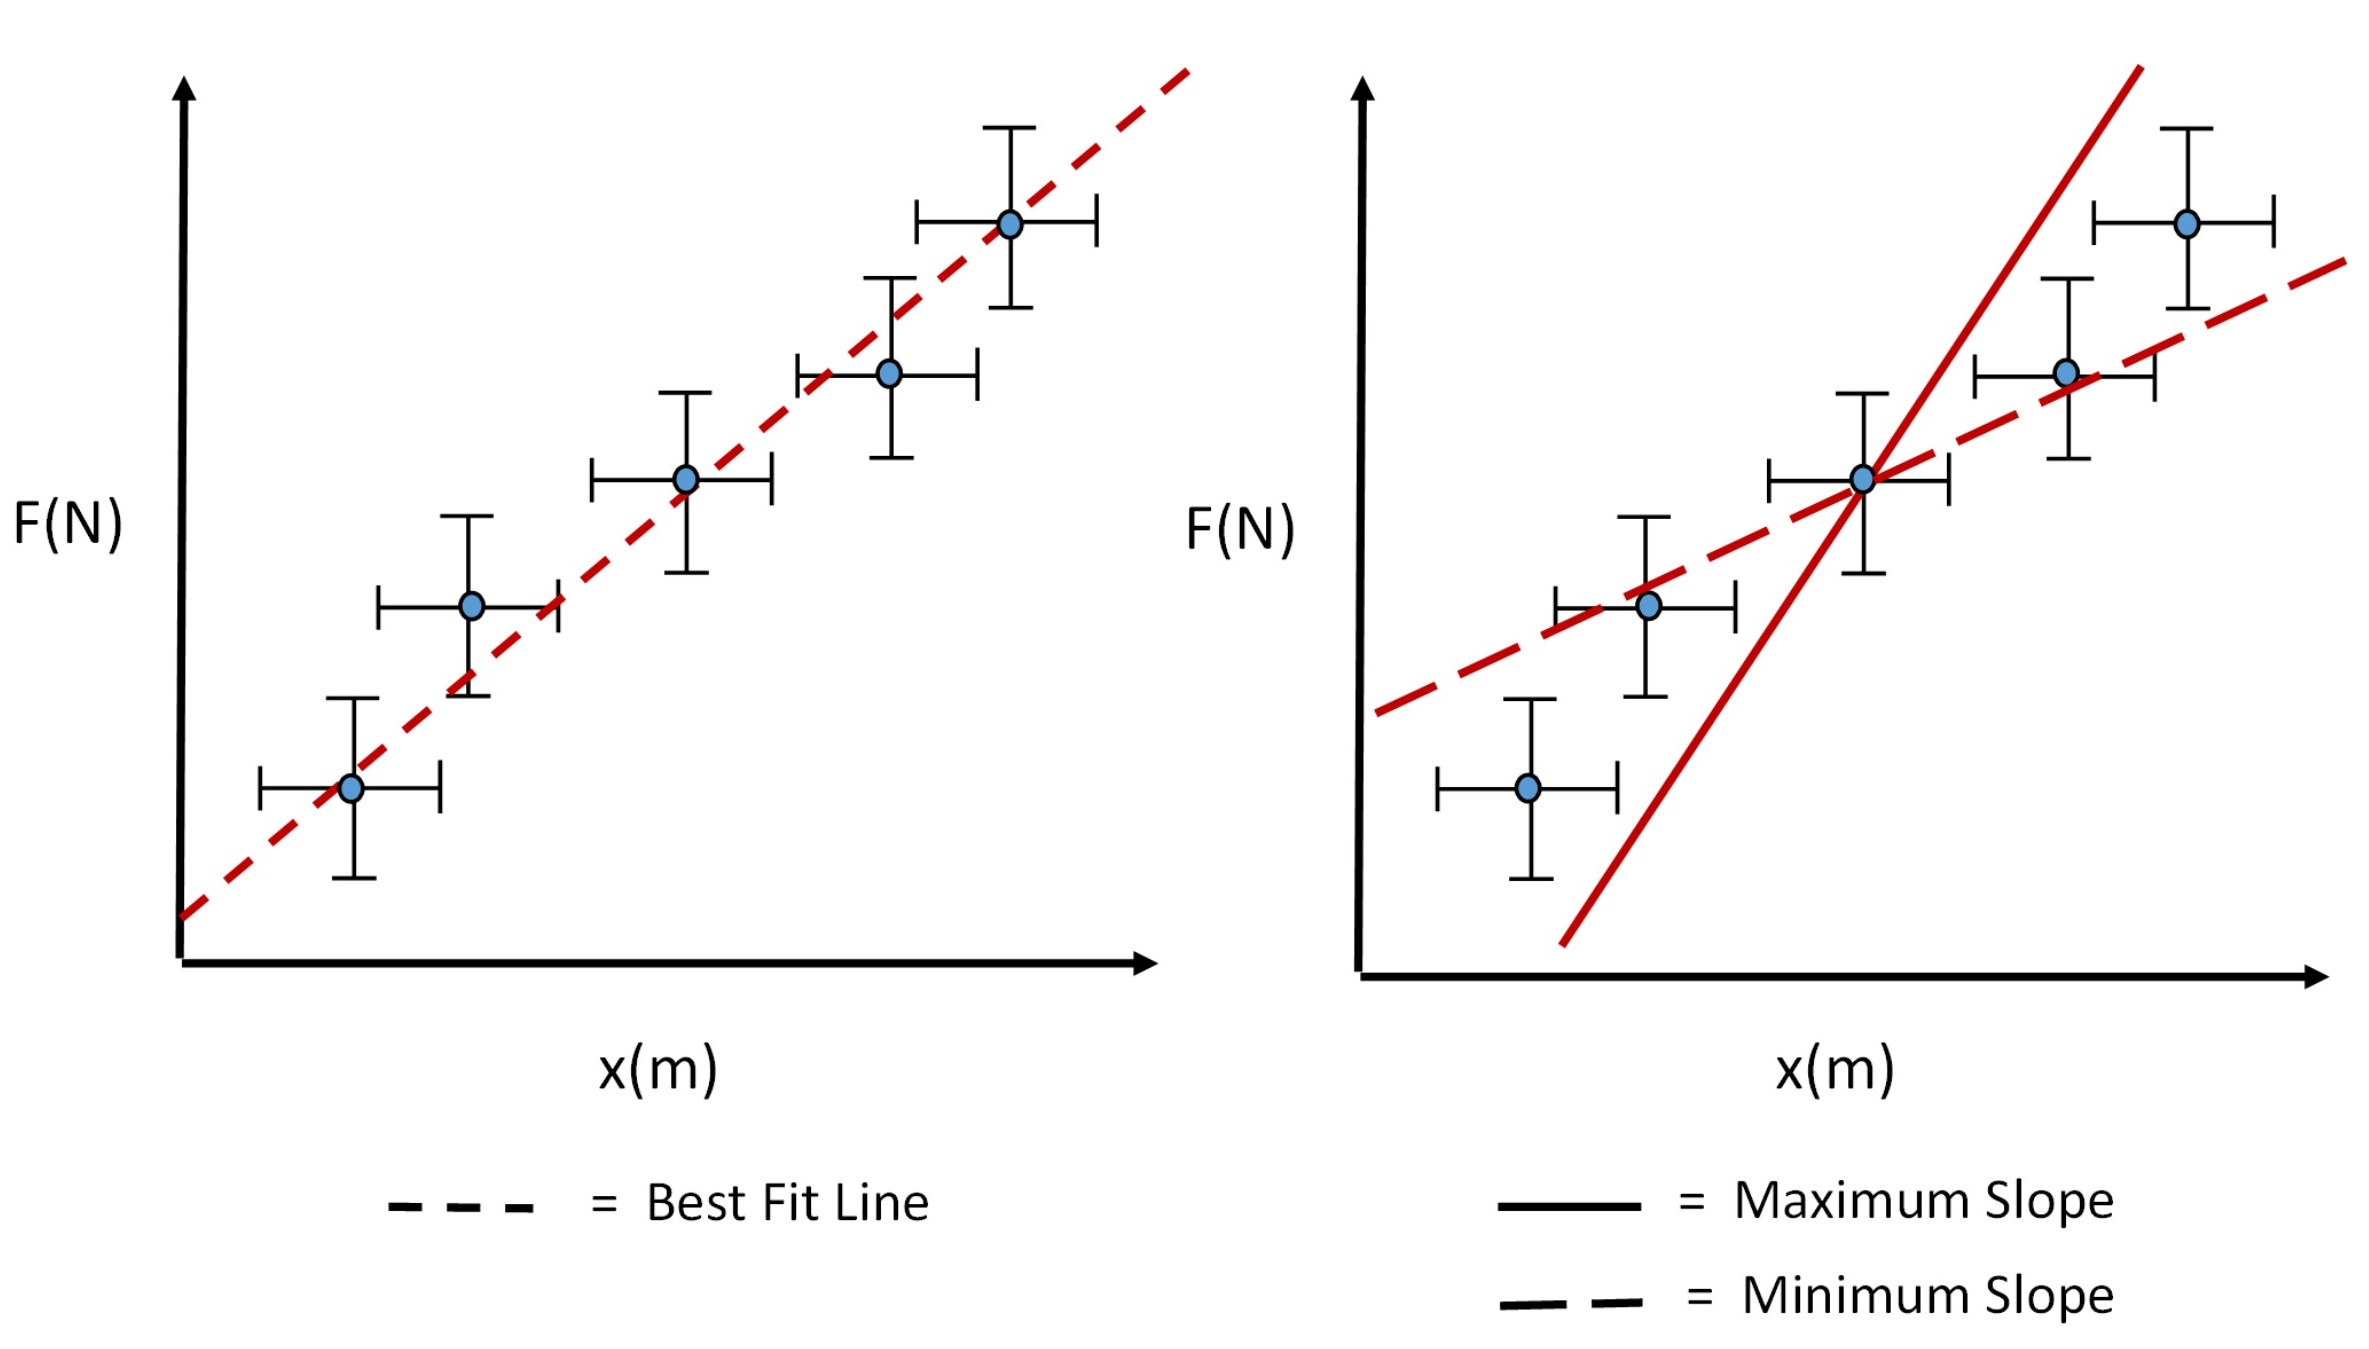
\includegraphics[width=0.9\textwidth, height=0.5\textwidth]{./Exp3/pic/image13.jpg}
    \end{center}
    \caption{Left: an example best-fit line. Right: the maximum and minimum possible slope from our data used to calculate uncertainty in the best-fit line. Notice how we have drawn the lines on the outer bounds of the error bars to achieve the maximum and minimum possible slope within the error bars.}
    \label{fig:bestfit}
\end{figure}

How do we know which line represents the best fit?  There is actually an exact mathematical procedure to obtain the best-fit line, but since this is a tedious calculation (and usually done on a computer), we will introduce some useful ``eyeball'' methods that can be done easily (without a computer). These techniques are sufficiently precise for our purposes, and with some experience they give results surprisingly close to the best fits produce by computer algorithms. \myskip

How does one draw the best line?  First, try to draw a line with as many points (with uncertainties included) lying above the line as below it. The gauge of how close the line is to a point is given by the uncertainty associated with that measured point. However, all the points at the left end should not lie on one side of the line with all the points at the right end lying on the other side. As a rule of thumb, roughly 2/3 of the points should have the line passing through the uncertainties (just as with the 2/3 rule).\myskip
%The uncertainty for the best-fit line is obtained by estimating how much one could increase and decrease the slope of the line before the fit is deemed very bad. \myskip

Clearly, this ''eyeball'' method has inherent uncertainty, so how do we estimate the uncertainty on the slope of the best-fit line? To do this we should estimate the spread of the slope, or maximum and minimum possible slopes that one can conceivably interpret from the graph. Half the difference between the minimum and maximum slopes is a good estimate of the slope uncertainty ($\sigma=\frac{m_{max}-m_{min}}{2}$). See figure \ref{fig:bestfit} for an example bist fit line and max/min slopes for some sample data.  \myskip

\underline{Remark}: Often in our experiments the data points will not look as nice as in the above examples. One or several points may not be close to any best-fit line you try. Such anomalous points may occur, for example, because of a mistake in measuring. In such cases, it is acceptable to ignore these anomalies when estimating the best-fit line. (Of course you must note this fact down in your lab report)  Dropping anomalous points must be done with extreme care and only rarely (if you know the point is not physically meaningful).\footnote{More than once, data points that did not behave as theory predicted turned out to be new effects and led to Nobel prizes!}  It is better to choose a line with as many points above the line as below. If you are not sure of your measurements, it is better to re-measure or to take more data points. \myskip

\subsection{Plotting in Excel}
An important set data analysis tools in excel are plotting and linear fit functions. You will need to plot and fit data many times throughout this lab course, so make sure you are familiar with this section. Below is a walkthrough of plotting and fitting a set of data with error in excel. 
\begin{enumerate}
\item Before plotting, you need to have 4 columns with data: x data, y data, x error data, and y error data. Make sure you have entered the information into excel.
\item First select your x data and y data (you can select multiple boxes in excel by holding down the ctrl button while selecting). Make sure to select your x data first or your x and y axes will be switched.
\item Choose the subheading "insert", then "Scatter", then "Scatter with straight lines and markers". Now your x and y data should be plotted without error bars (see figure \ref{fig:excel1}).

\begin{figure}[h!]
\centering
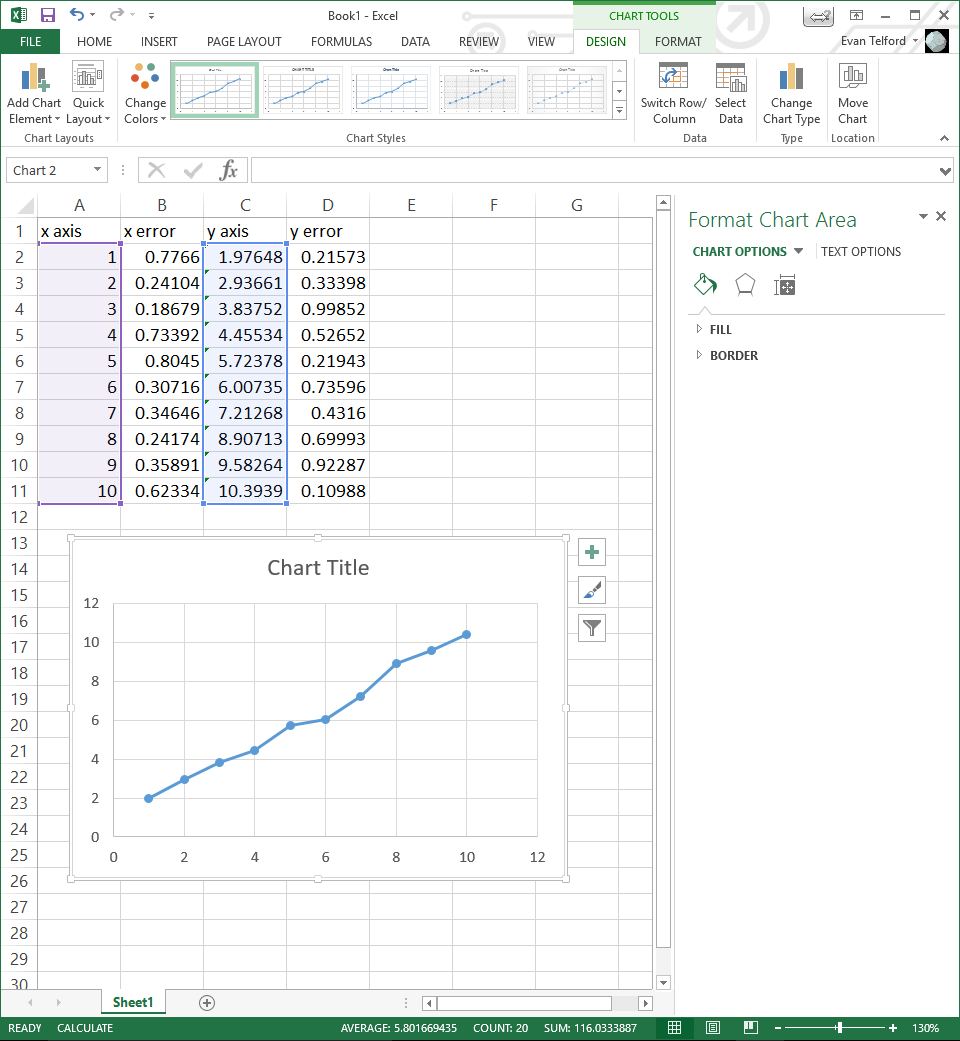
\includegraphics[height=0.4\textheight, width=0.7\textwidth]{./Exp1/pic/image4.png}
\caption{Selecting x and y data and creating a lined scatter plot in excel.}
\label{fig:excel1}
\end{figure}


\item To include error bars select your chart, then click the "plus" marker on the top right of the chart. Check the box titled "error bars". Now some basic error bars should appear on the plot. These are not based on the error bar data in your excel document, they are standard error bars.
\item To change them so they match your error bar data, select the x axis error bars on your chart, and format the error bars by clicking the "Custom" selection, then "specify value".
\item It should now prompt you for positive error values and negative error values. Delete "$\{1\}$" from the two boxes, and select your error bars using the cursor. Your chart will now have the correct error bars (see figure \ref{fig:excel2}).

\item Repeat steps 5-6 for your y data.
\item To linear fit your data, right click on your data in the plot and select "Add Trendline". Check the "Linear", "Display Equation on chart", and "Display R-square value on chart" boxes. 
\item Now the slope, intercept, and R squared values will be displayed on your chart. R squared is a measure of how well the line fits your data. It should be close to $1$ and at the very least greater than $0.9$.
\end{enumerate}

\begin{figure}[h!]
\centering
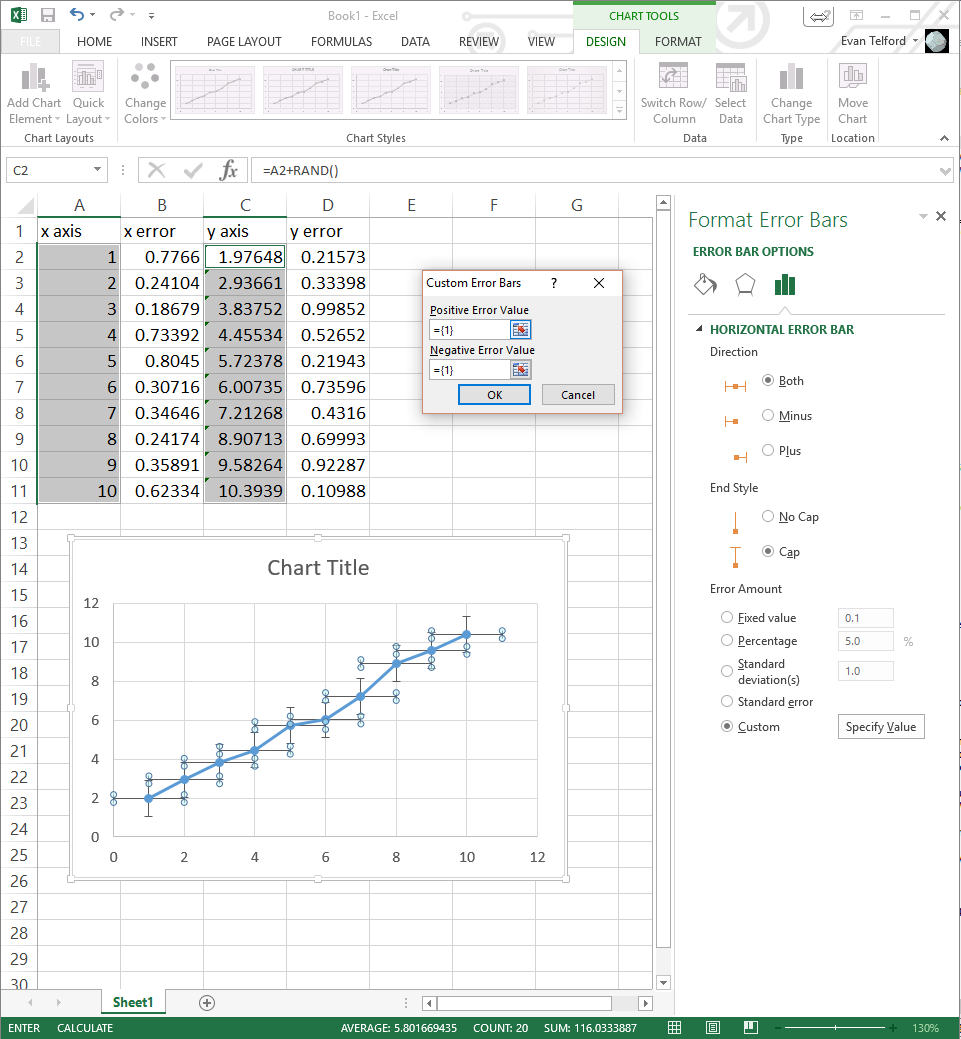
\includegraphics[height=0.4\textheight, width=0.7\textwidth]{./Exp1/pic/image5.png}
\caption{Using your own data set to create x and y error bars in excel.}
\label{fig:excel2}
\end{figure}

\begin{figure}[h!]
\centering
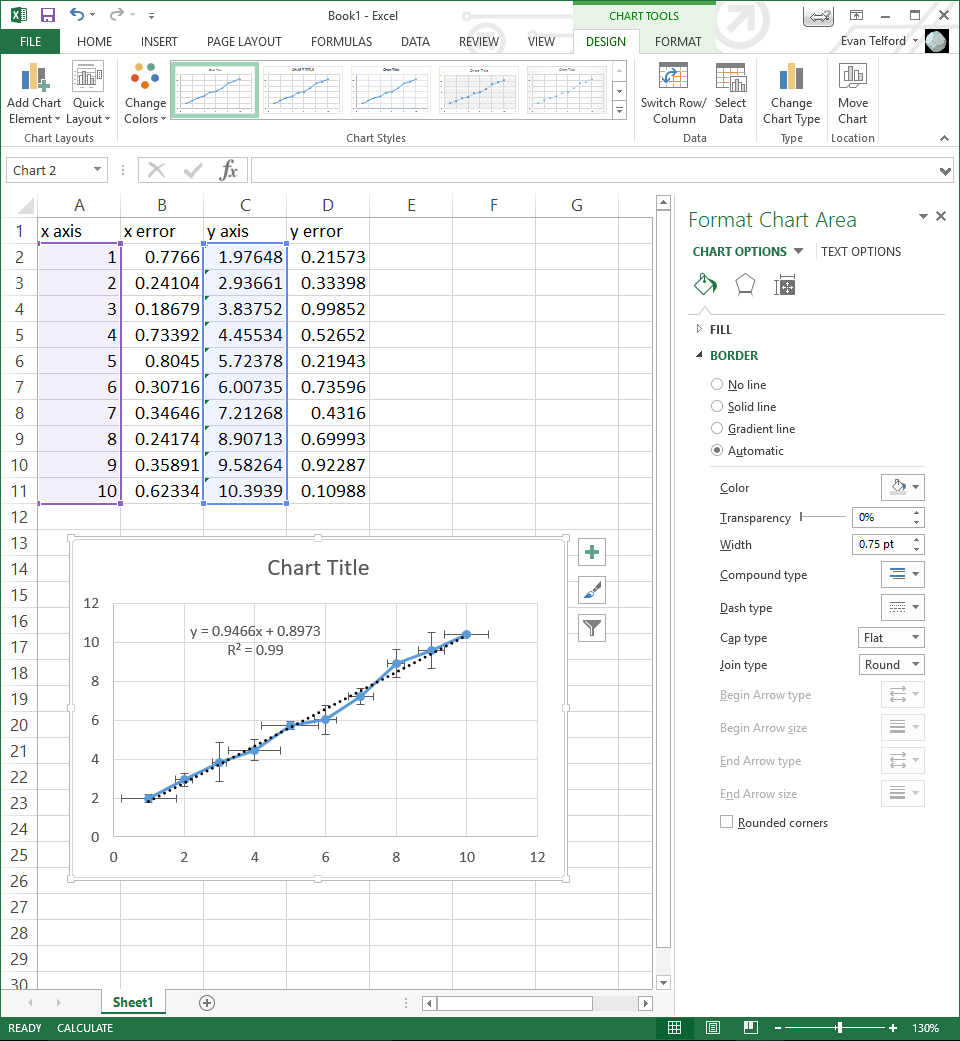
\includegraphics[height=0.4\textheight, width = 0.7\textwidth]{./Exp1/pic/image6.png}
\caption{Using excel to perform a linear fit and return the intercept and slope.}
\label{fig:excel3}
\end{figure}
\newpage
\subsection{Simple Pendulum}
In this experiment, we will study the dynamics of a simple pendulum. A simple pendulum is defined as a small mass (known as a pendulum bob), treated as a point mass, suspended from a thin wire considered to be massless. When displaced from equilibrium, the mass will oscillate around the equilibrium point. To analyze the mechanics of the simple pendulum, we use Newton's second law to examine the forces on the pendulum bob (see figure \ref{fig:pendulum}).
\myskip
Looking at figure \ref{fig:pendulum}, we can write down Newton's second law.
\begin{gather}
F = -mg\sin(\theta) \\
F = ml \frac{d^2}{dt^2}\theta \\
\text{using the small angle approximation} \hspace{3mm} \sin(\theta) \sim \theta \nonumber \\
-\frac{g}{l} \theta = \frac{d^2}{dt^2}\theta
\end{gather}
You may recognize equation 2.8 as the equation for simple harmonic motion. In simple harmonic motion, the object (in this case the pendulum) will oscillate about an equilibrium point with a specific frequency $f$. The frequency can be found from Newton's second law as simple harmonic motion takes the following form.
\begin{gather}
-(2\pi f)^2 \theta = \frac{d^2}{dt^2}\theta
\end{gather}
By comparison of equations 2.8 and 2.9, the frequency can be determined in terms of know parameters.
\begin{gather}
f = \frac{1}{2\pi}\sqrt{\frac{g}{l}}
\end{gather}
In experiment, we can more easily measure the period of oscillation, which is related to the frequency $\tau = 1/f$. Therefore, we also have an expression for the period of oscillation in terms of know parameters.
\begin{gather}
\tau=2\pi \sqrt{\frac{l}{g}}
\end{gather}

\begin{figure}[h]
\centering
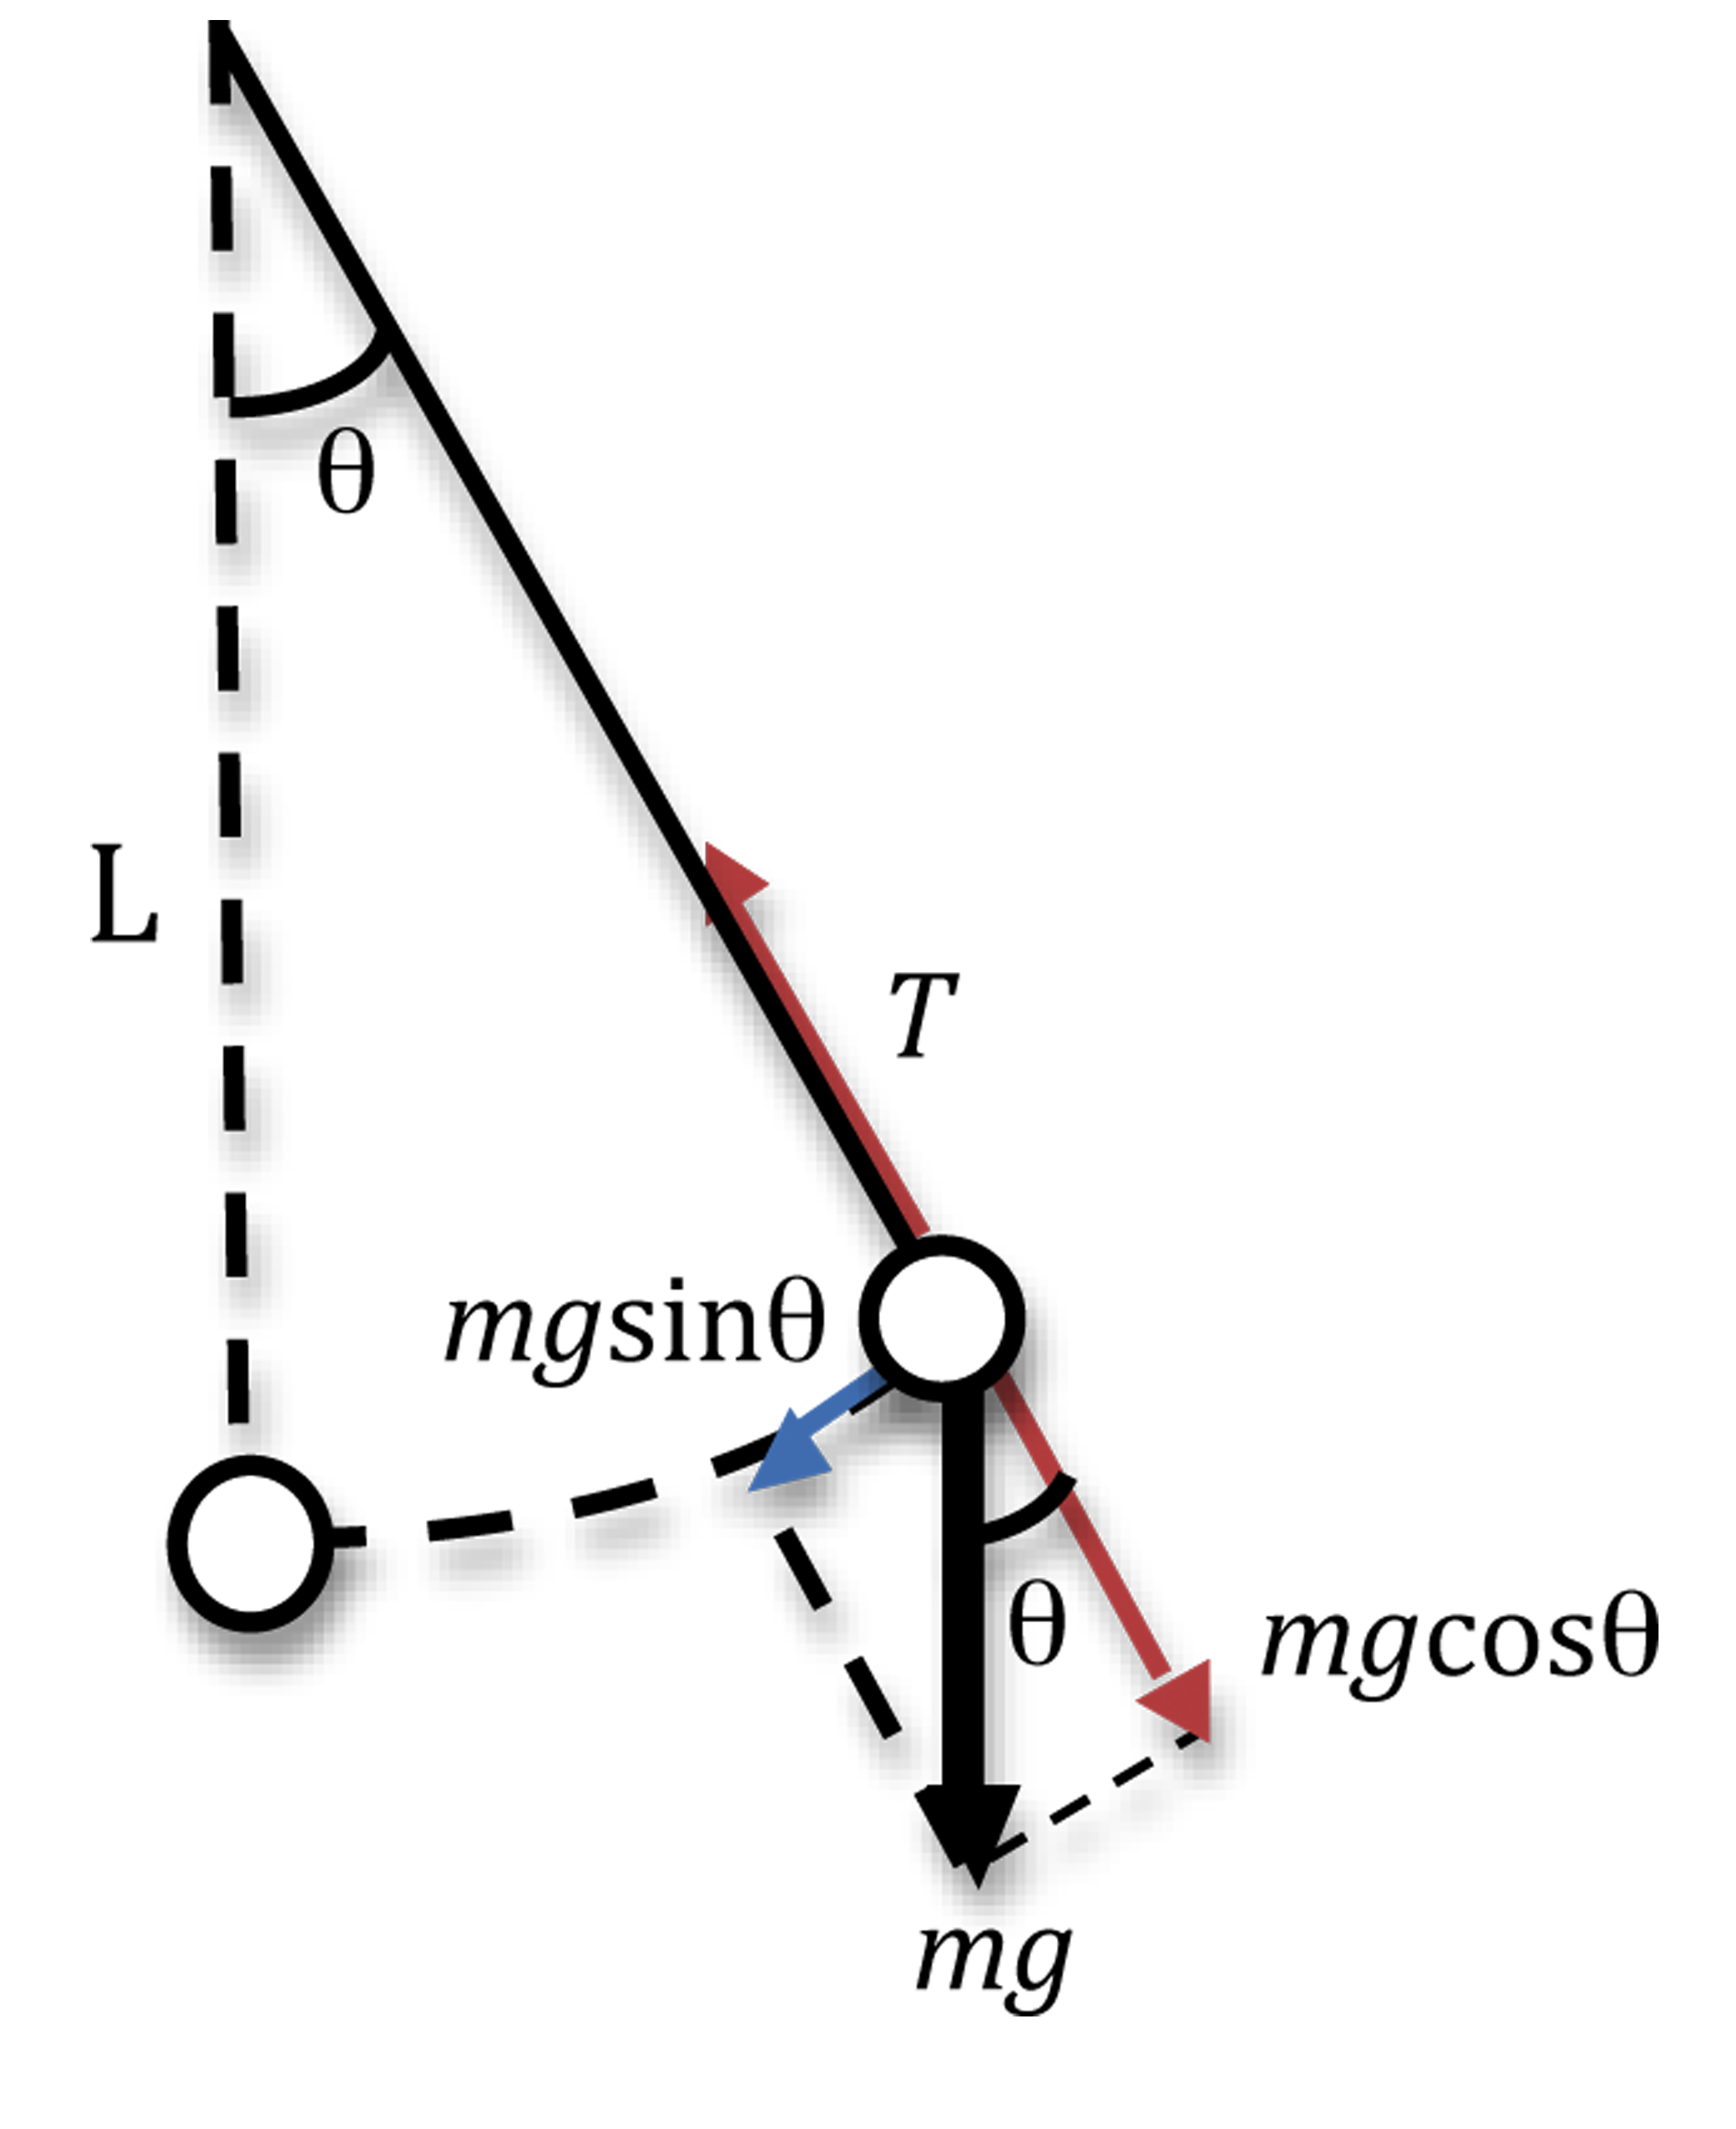
\includegraphics[width=0.5\textwidth]{./Exp1/pic/pendulum.png}
\caption{A free body diagram of a simple pendulum undergoing simple harmonic motion}
\label{fig:pendulum}
\end{figure}

\newpage
\subsection{Buffon's Needle}
Buffon's needle problem is a classic probability problems first posed by Georges-Louis Leclerc, Comte de Buffon that we will reproduce in this lab. It is stated as follows.
\begin{quotation}
"Suppose we have a floor made of parallel strips of wood, each the same width, and we drop a needle onto the floor. What is the probability that the needle will lie across a line between two strips?"
\end{quotation}
If the needle is shorter than the distance between two strips, the solution is surprisingly simple. The probability of a needle landing on a line is given by the following formula.
\begin{gather}
P = \frac{2 L}{D \pi}
\label{equ:buffon}
\end{gather}
Where $L$ is the length of a single needle and $D$ is the distance between lines. The original question posed was trying to calculate the probability of needle falling between two lines, however, it is more interesting to use the derived relation to calculate the numerical value of $\pi$. We can do so by performing the following experiment.
\begin{enumerate}
\item Begin by drawing parallel lines one a sheet of paper and measuring the distance between the lines.
\item Drop a preset number of "needles" (usually toothpicks with a well defined length) and calculate the probability $P$ by dividing the number of needles that land on a line by the total number of dropped needles.
\item From $P$ you can calculate $\pi$.
\end{enumerate}
For a more detailed derivation and description of the problem, visit this online article on \href{https://en.wikipedia.org/wiki/Buffon\%27s_needle}{Buffon's needle} \footnote{https://en.wikipedia.org/wiki/Buffon\%27s\_needle}. For an extension of the problem to objects other than needles, visit this online article on \href{https://en.wikipedia.org/wiki/Buffon\%27s_noodle}{Buffon's noodle} \footnote{https://en.wikipedia.org/wiki/Buffon\%27s\_noodle}. A schematic is given in figure \ref{fig:buffon}.

\begin{figure}[h]
\centering
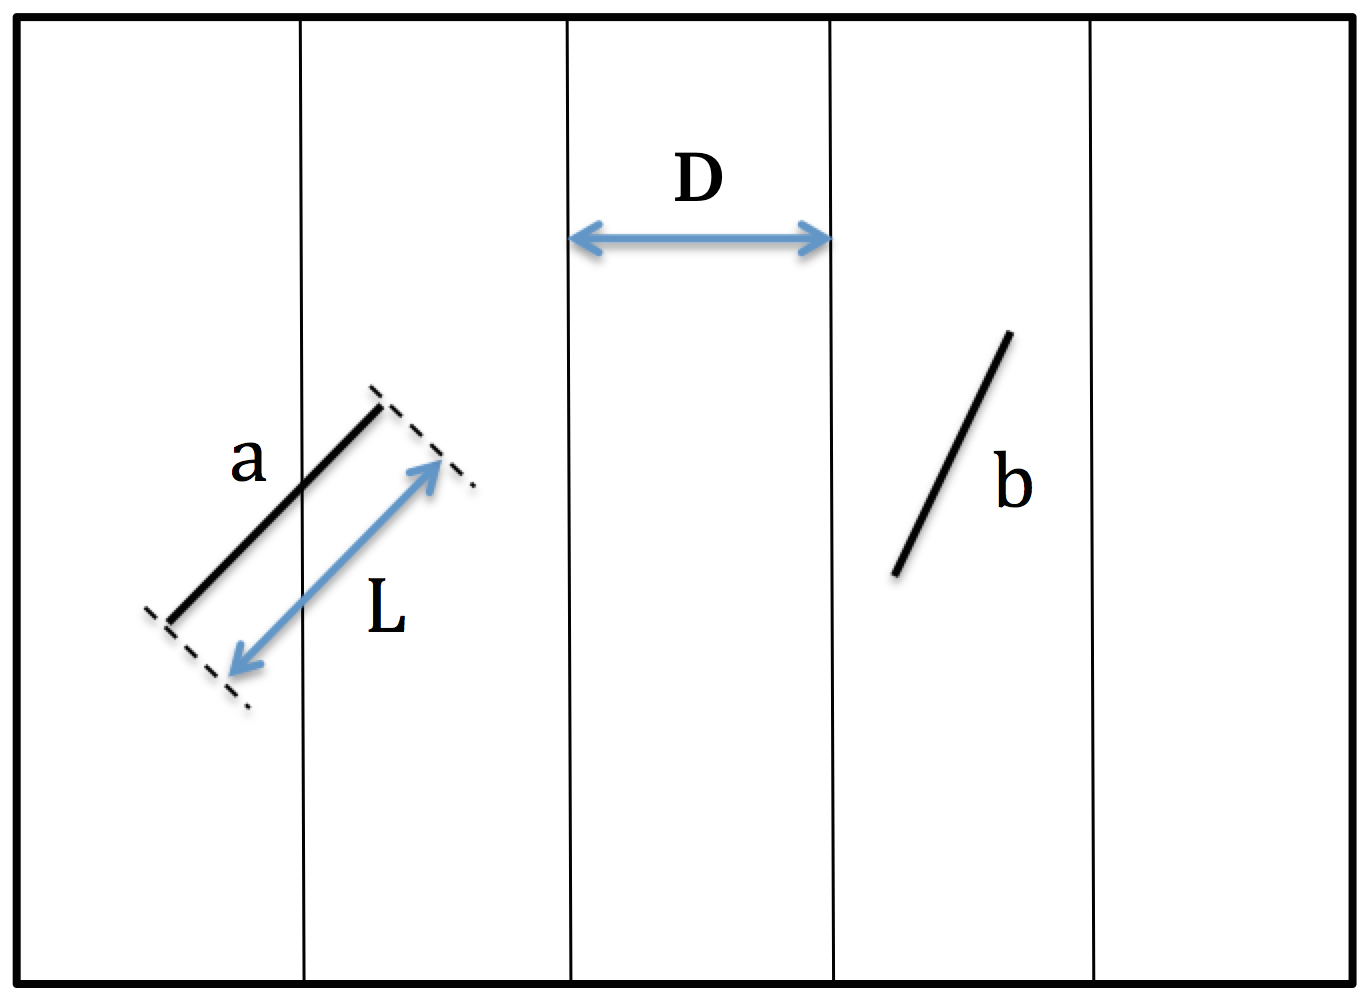
\includegraphics[width=0.7\textwidth]{./Exp1/pic/buffon.png}
\caption{A schematic of Buffon's needle experiment. The distance between lines is $D$ and the length of a single needle is $L$.}
\label{fig:buffon}
\end{figure}

\section{Procedure}
\subsection{Pendulum}

In the first part, you will determine the gravitational constant $g$ through two methods. First, you will measure the time it takes a pendulum to swing through a full cycle, the period of oscillation, and use this to calculate the gravitational constant $g$. Second, you will measure the period for 5 different pendulum lengths and use the linear fit method to determine the gravitation constant $g$.. Since a number of measurements need to be made, you may wish to perform this experiment in teams of two: one person measures the time values, the other records the results. \myskip

\begin{itemize}
\item Measurement 1: Calculation of $g$ by measuring multiple periods $\tau$.
\begin{enumerate}
\item Begin by measuring the length of the pendulum with error and recording it in your report.
\item Let the pendulum swing at some small angle (less then 15 degrees) and measure the period of the motion. Try to start and stop the stopwatch at the apex of the motion. A full period is the time it takes to travel from one maximum point to back to the same point. Take 18 measurements of the period and record the data in an excel document.
\item Use excel functions to determine the error in measured period using two methods: first, calculate the standard deviation, then estimate the error using the 2/3 method. Do the two methods give a similar error? Use standard deviation as the error in later calculations.
\item Use the following formula to determine the gravitational constant $g$ with error found by propagating uncertainties in pendulum length $l$ and period $\tau$.
\begin{gather}
 \frac{2\cdot \pi}{t} = \sqrt{\frac{g}{\ell}}
\end{gather}
\item Does your calculated value of $g$ agree with the expected value ($g=9.81 m/s^2$)?
\item What are the major sources of error in this part of the experiment?
\end{enumerate}
\item Measurement 2: Calculation of $g$ by measuring the period as a function of pendulum length.
\begin{enumerate}
\item Measure the length of the pendulum with error and record it in your report.
\item Let the pendulum swing at some small angle (less then 15 degrees) and measure the period of the motion. Try to start and stop the stopwatch at the apex of the motion. Make a single measurement of the period $\tau$.
\item repeat steps 1-2 for 5 different pendulum lengths $\ell$. 
\item In excel, plot the length of the pendulum $\ell$ versus period squared $\tau^2$ with error bars on both axes. The error bars in $\ell$ and $\tau$ can be determined from the precision in the ruler/stopwatch (make sure to correctly propagate the error in squaring $\tau$).
\item Use excel to fit your plot with a line and use the generated slope to determine the gravitational constant $g$. Include error in $g$ using the max-min method for linear fit error (discussed in section 2.1.3) (We suggest printing out your excel plot and doing the max-min method by hand).
\item Does your calculated value of $g$ agree with the expected value?
\item What are the main sources of error in this part of the experiment?
\end{enumerate}
\end{itemize}
\subsection{Buffon's Needle}
In this experiment, you will determine the value of $\pi$ through Buffon's probability experiment (see section 2.2 for a detailed explanation). You will need a piece of paper and the toothpicks provided in the lab.
\begin{enumerate}
\item Measure the length of a single toothpick and record it in your report with error.
\item Draw at least four parallel lines on a piece of plain printer paper. Make sure all lines are equidistant apart {\it{and}} the distance between lines is greater than the length of a single toothpick. Record the distance between lines in your report with error.
\item Drop 10 toothpicks on your piece of paper and record the number of toothpicks that cross a line with error.
\item Calculate the value of $\pi$ (using equation \ref{equ:buffon}) with error found by propagating uncertainties in measured lengths and the number of counts.
\item Repeat steps 3-4 this time dropping 50 toothpicks.
\item Do your calculated values of $\pi$ agree with the expected results ($\pi = 3.14159...$).
\item In which trial did you calculate a more accurate value of $\pi$. In which trial did you calculate a more precise value of $\pi$? Is this expected?
\end{enumerate}
(Optional) For those of you who are interested in a more in depth analysis of this experiment, you can try and work through the next two bullet points.
\begin{enumerate}
\item Buffon's needle experiment can be improved by using objects other than toothpicks such as triangles, circles, v shaped toothpicks, etc... where the number of counts is still the number of times a line is intersected by the dropped shape. Use the online Buffon's needle simulator \href{http://mste.illinois.edu/activity/buffon/}{here} \footnote{http://mste.illinois.edu/activity/buffon/} to determine which shape determines the most accurate value of $\pi$ in the fewest number of drops (make sure to use a "needle scale" of $1$). 
\item Why might the shape you found in the previous part give you the most accurate value of $\pi$?
\end{enumerate}


\section{Lab Preparation Examples}

\myskip
{\bf{Note: Suggested prelab questions are in bold. These will help with conceptual under- standing of the laboratory experiments. }}
\myskip

\noindent \underline{Estimation of Uncertainty}:\myskip

1. You have the following distribution of measured values:
\begin{table}[h]
    \centering
    \begin{tabular}{|c|l|l|l|}
        \hline
         %& 5 & 10 & 15 \\ \hline
        \quad 0\quad & \hspace{1.5cm} & \hspace{1.5cm} & \hspace{1.5cm} \\ \hline
        \quad 1\quad & I & \hspace{1.5cm} & \hspace{1.5cm} \\ \hline
        \quad 2\quad & III & \hspace{1.5cm} & \hspace{1.5cm} \\ \hline
        \quad 3\quad & IIIII & I & \hspace{1.5cm} \\ \hline
        \quad 4\quad & IIIII & IIII & \hspace{1.5cm} \\ \hline
        \quad 5\quad & IIIII & IIIII & IIIII \\ \hline
        \quad 6\quad & IIIII & IIIII & I \\ \hline
        \quad 7\quad & IIIII & III & \hspace{1.5cm} \\ \hline
        \quad 8\quad & IIII & \hspace{1.5cm} & \hspace{1.5cm} \\ \hline
        \quad 9\quad & II & \hspace{1.5cm} & \hspace{1.5cm} \\ \hline
        \quad 10\quad & I & \hspace{1.5cm} & \hspace{1.5cm} \\ \hline
    \end{tabular}
\end{table}

Estimate the uncertainty using the 2/3 estimate. \myskip

2. Estimate the mean and uncertainty of the following group of values:
\begin{equation*}
    1.6\,\mathrm{s}, 1.3\,\mathrm{s}, 1.7\,\mathrm{s}, 1.4\,\mathrm{s}
\end{equation*}

3. In a radioactive decay you get 16 counts. What is the absolute uncertainty of the number of counts? What is the relative uncertainty? \myskip

4. In a radioactive decay you get 1600 counts. What is the absolute uncertainty of the number of counts? What is the relative uncertainty? \myskip

{\bf{5. How many counts should you get so that the relative uncertainty is $1\%$ or less? }}\myskip

\noindent \underline{Significant digits}: \myskip

6. How many significant digits has $l = 0.0254\,\mathrm{m}$? \myskip

7. Write $t = 1.25578 \pm 0.1247\,\mathrm{s}$ with two significant digits (in the uncertainty). \myskip

\noindent \underline{Propagation of Uncertainty}: \myskip

{\bf{8. For a pendulum with $l = 1.0 \pm 0.1\,\mathrm{m}$, you measure a period of $t = 2.0 \pm 0.2\,\mathrm{s}$. What is the value of the earth's acceleration g?}} \myskip

{\bf{9. You measure the volume of a box by measuring the length of the single sides. For the lengths of the single sides you get:
\begin{equation*}
    a = 10.0 \pm 0.1\,\mathrm{cm}\qquad    b = 5.0 \pm 0.2\,\mathrm{cm} \qquad c = 7.5 \pm 0.3\,\mathrm{cm}
\end{equation*}
What is the volume of the box (including uncertainty and units) in $\mathrm{cm}^3$? What is the volume of the box in $\mathrm{m}^3$? }}\myskip

10. You measure the following quantities:
\begin{align*}
    A &= 1.0 \pm 0.2\,\mathrm{m}\quad B = 2.0 \pm 0.2\,\mathrm{m}\quad        C = 2.5 \pm 0.5\,\mathrm{m/s} \\ 
    D &= 0.10\pm 0.01\,\mathrm{s}\quad E = 100\pm 10\,\mathrm{m/s^2} &
\end{align*}
Calculate the mean and uncertainty of:
\begin{enumerate}[a)]
    \item $A+B=$
    \item $A-B=$
    \item $C\cdot D=$
    \item $C/D=$
    \item $C\cdot D + A=$
    \item $\frac{1}{2}E\cdot D + C=$
    \item $A\cdot B/(A-B)=$
\end{enumerate}
Include units! For e)--g) perform it step by step.\myskip

\noindent \underline{Relative and Absolute Uncertainty}:\myskip

11. What is the relative uncertainty for $v = 12.25 \pm 0.25\,\mathrm{m/s}$?\myskip

12. What is the absolute uncertainty if the mean value is $120\,\mathrm{s}$ and the relative uncertainty is $5\%$?\myskip

{\bf{13. Given the following measurements, which one has the highest absolute uncertainty and which one has the highest relative uncertainty?}}
\begin{align*}
    l &= 10.0 \pm 0.2\,\mathrm{m} \quad   l = 10.0\,\mathrm{m}\: (1.00 \pm 0.03)   \\ 
    l &= 7.24\,\mathrm{m}\: (1.00 \pm 0.04) \quad l = 12.5 \pm 0.25\,\mathrm{m}   
\end{align*}

14. Given the following measurements which one has the highest absolute uncertainty and which one has the highest relative uncertainty?\myskip
\begin{align*}
    l &= 10.0\pm 0.2\,\mathrm{m} \quad t = 7.5\pm 0.2\,\mathrm{s} \\
    d &= 5.6\,\mathrm{cm}\:(1.00\pm 0.04) \quad v = 6.4\times 10^6\,\mathrm{m/s}\:(1.00\pm 0.03)
\end{align*}
\emph{Caution}: Don't get tricked!\myskip

\noindent \underline{Explanations}:\myskip

{\bf{15. Explain, using your own words, why the uncertainty decreases as you average over several measurements (you might want to take a look at the appendix).}} \myskip

%16. Explain, using your own words, the difference between uncertainty and error as you perform several measurements and average.\myskip

16. You measure the speed of light and get as a result $c = (2.25 \pm 0.25)\times 10^8\,\mathrm{m/s}$. The value you find in books is $c = 299\, 792\, 458\,\mathrm{m/s}$.  Using these values explain the difference between the uncertainty of your measurement and its error!

